\chapter{関連研究}
\label{chap:previous}
\fancyhf{}
\rhead{\thepage}
\lhead{第\ref{chap:previous}章 関連研究}
\cfoot{\thepage}


本研究が問題提起を行った知識獲得予測の研究は,
%今日の教育を取り巻く環境や,
学習科学の発達や,
教育に関する大規模分析の活発化,
深層学習技術やその他の多様な分析技術の進展により発展してきた研究分野である.
本章では,知識獲得予測の関連研究を俯瞰し,
現状の環境や周辺概念を整理することで,本研究の学術的位置づけを明確にする.


%まず,教育の個人最適化に関する現状や研究について整理した後,
まず,人間の学習効果について研究する学習科学の歴史と情報技術の発達との関係性について整理した後,
その情報技術の一つとして,教育の個人最適化を解決すると期待されているオンライン教育サービスについて,具体的な事例を挙げながら,その効果や関連する研究について述べる.
次に,深層学習について概説し,本論文との関わりが深いRecurrent Neural Netoworksについて詳細に述べる.
さらに,知識獲得の予測手法であるKnowledge Tracingについて,その有益性や,伝統的な手法,深層学習を用いた最先端の手法について整理した後,
本研究において既存手法を拡張する上で用いる,大規模データから次元削減を行う関連手法について整理する.
最後に,以上の関連研究を踏まえて,
本論文で使用する類似の用語について,定義を明確にする.


\section{学習科学と情報技術}

%学習科学(Learning Sciences)という言葉は,1991年にThe Journal of The Learning Sciencesの国際会議で登場した学問分野である[参考文献引用].
20世紀後半,人間の心の働きを理論化する認知科学が,現実社会で実際に役立つ科学として再構築される流れの中で,
人を日常の学びの中で今より賢くするために実際に役立つ科学として,「学習科学(Learning Sciences)」の分野が確立された\cite{白水始2014学習科学の新展開}.
学習科学は,従来の,実験室環境でのみ確認されるような非実用的な理論研究を避け,
学習がうまくいく要因や状況を解明した上で,その学習を人間が積極的に引き起こすことを目指すような,実践の学を新たに打ち立てることを目指したものであった.
明確な定義は様々であるが,\cite{三宅なほみ2002学習環境のデザイン実験}らは2002年に
「よりよい教育を実現したいという社会的要請を背景にして,これまでの認知研究に基づき,
現実の人の学習,例えば学校教育の中での子どもたちの学習を研究し,
現代のテクノロジを駆使して実効性のある教育のシステムを教育実践の中で作り上げようという研究動向」
と定義している.


学習科学の発展は,
認知科学の進展だけでなく,情報技術の発達が大きな貢献を果たしている.
学習科学は,人間の認知過程を解明する基礎研究としての性質に加え,
実社会での有効性を検証する実証的な応用研究としての性質を兼ね備えているため,
オンライン教育サービスのような教育と情報技術の融合によって,
これまで実現しにくかった学習環境を作り検証できるようになったことは,
学習科学の発展を大きく加速させた.

そうした情報技術との融合により実証研究が進み,今日注目されている分野の例として「アダプティブラーニング」が挙げられる\cite{carbonell1970ai, midgley2014goals}.
アダプティブラーニングは,個人に最適化された学習内容の自動提供を実現するもので,
その社会的影響の大きさからアメリカを中心に注目が集まっており,関連するスタートアップや大学での研究に,多額の資金が投入されている\cite{piccioli2014learning}.

学習内容を個人に最適化させるという考え自体は,
学習科学研究の分野でも,また,研究という形に上がらないレベルでも,古くから存在し,
例えば習熟の遅い生徒に教師が個別で補習に当たったり,
個別指導塾や通信教育で生徒各自が自身の習熟度にあった講義を受けたりと,
様々な形態を取って実践されてきた.
しかし,こうした従来の方法は,
教育の粒度を細かくし,個人最適化を図ろうとするほど,
教師一人あたりが担当できる生徒の数が減ることによる人材的・金銭的負担や,
教師ごとの指導能力の違いなどの問題に直面し,
誰もが平等に最適な教育を受けるという目的を達成するには,障壁が残っていた.

この事態を打開したのが,教育と情報技術の融合である.
中でも,その象徴とも言えるオンライン教育サービスでは,
サービスを利用する生徒の学習行動ログを収集することで,
これまで困難であった大規模な学習効果分析を可能にしたことに加え,
オンライン上の学習コンテンツを生徒が個人で利用するという形態を活用し,
研究成果を元に学習コンテンツを個人に最適化して提供することを容易にした.


このように,基礎理論に加え実証性も重視する学習科学の領域は,
情報技術との融合により大きく発達してきた.
特に,オンライン教育サービスは,
データの蓄積と研究成果の実証という二つの目的が達成できるプラットフォームとして,
大きな注目を集めている.



以上,学習科学と情報技術の関係性について述べた.
次に,教育と情報技術の融合を象徴する例として,オンライン教育サービスについて述べる.




\section{オンライン教育サービスと大規模な学習効果分析}
オンライン教育サービスの代表的な例としてMassive Open Online Courses(MOOCs)とIntelligent Tutoring System(ITS)を取り上げ,
具体的な事例を挙げながら,関連する研究について述べる.
また,こうしたオンライン教育サービスが大規模分析に活用されている状況や研究について整理する.


\subsection{MOOCsとITS}
MOOCsはMassive Open Online Courses\cite{mcauley2010mooc, pappano2012year,siemens2013massive}の略称で,
特に日本語で表記する場合は大規模公開オンライン講座と記述することがある.
MOOCsは,オンライン上で公開された,大学を始めとする様々な教育機関などの講座を,誰もが無償で受講でき,また修了時には修了証も取得できる教育サービスのことを指す.

学びたい人が,いつでもどこでも学習リソースにアクセスできるというMOOCsの概念自体は古くから提唱されていたが,
実現化したのは,2008年にカナダのマニトバ大学で学生向けのオンライン講座を開設した際に,
25人の受講者だけでなく2000人以上の人がその講座に参加したことがきっかけだと言われている\cite{yuan2013moocs}.

以前から,大学などの高等教育機関は,
オープンコースウェア\cite{abelson2008creation}という形で講義の動画や資料を公開していたが,
MOOCsは,参加人数が非常に大規模で,また,高等教育水準の内容だけでなく,初等中等教育水準の内容の講座も含まれている点で異なる.
また,これまでもオンラインの講座というものは存在していたが,
MOOCsは,
参加人数が非常に大規模である点や
公開している講座の数が大規模である点,
また,その内容が多様であるという点,
利用が無料,あるいは無料に近いという点において,
これまでのオンライン講座とは異なる.


MOOCsは,従来の,学校の教室で一斉授業形式で提供される教育形態と異なり,
オンライン上の多様な講座に,生徒が個人でアクセスし,
講座ごとに提供される講義の動画や演習システムなどを通じて,
いつでもどこでも,自身の習熟度合いやペースに合わせて,自分の学習したいものを選択して学習できる.
従来の教育の,生徒が自身の習熟度合いに見合った学習ができないという問題を解決するものとして注目されていることに加え,
産業や社会への影響も注目されている.
例えば,大学生だけでなく社会人も,自身の専門領域に関する講座を受講することでより理解を深めたり,
あるいは専門領域とは異なる幅広い講座を受講することで,教養を養うことができる.
また,公教育の整備が追いついていないような発展途上国においては,
MOOCsが教育に与える影響は大きく,その影響や可能性を分析する報告は多い\cite{trucano2013more,liyanagunawardena2013impact}.

このように,MOOCsは社会の多様な場面で,これまでにない学習機会を提供しており,
教育や学習といったもののあり方に大きな影響を与えている.


\begin{figure}[htb]
\begin{center}
%\hspace*{-40pt}\makebox[1.2\textwidth][c]{
\makebox[1.2\textwidth][c]{
	\minipage{0.53\textwidth}
		
\includegraphics[width=180pt]{./img/coursera.png}
		\caption{Courseraのイメージ}
		\label{fig:cousera}
	\endminipage\hfill
	\minipage{0.53\textwidth}
		
\includegraphics[width=180pt]{./img/jmooc.png}
		\caption{JMOOCのイメージ}
		\label{fig:jmooc}
	\endminipage\hfill
}
\end{center}
\end{figure}

MOOCsの有名な事例として,世界的に有名なCourseraや,日本発のMOOCsであるJMOOCが挙げられる.
CourseraとJMOOCのイメージを図\ref{fig:cousera},\ref{fig:jmooc}に示す.
Courseraは,2017年1月の時点で,
29の国にまたがる148の教育機関とパートナーシップを結び,
コンピュータサイエンス,数学や論理,社会科学などに関する1600以上の講座を,2200万人以上に提供している\footnote{講座数と利用者数はトップページの記載より引用.}.
JMOOCは,2013年11月に日本版のMOOCsとして設立され,
10代から80代までと幅広い年代に,アートや医療,自然科学や資格試験対策などの講座を提供しており,
2017年1月の時点で,140の講座を50万人以上が受講している\footnote{講座数と利用者数はトップページの記載より引用.}.


多様な講座を多くの人に提供するMOOCs以外にも,
より個人の学習過程をサポートすることを目的として設計された,
Intelligent Tutoring System(ITS)と呼ばれるオンライン自動学習支援システムの利用も拡大している\cite{sleeman1982intelligent}.

\begin{figure}[htb]
\begin{center}

\includegraphics[width=200pt]{./img/knewton.png}
\end{center}
\caption{Knewtonのイメージ}
\label{fig:knewton}
\end{figure}

ITSの有名な事例として,世界最大級のITSであるKnewton\footnote{\url{https://www.knewton.com/}}のイメージを図\ref{fig:knewton}に示す.
Knewtonでは,生徒の学力や理解度と,学ぶべき対象をマッピングすることで、
生徒に最適な学習過程を設計し,
かつ生徒の学習の進捗に応じてその過程を動的に変化させる仕組みを有している\cite{upbin2012knewton}.


また,近年では,これまで難しいと言われていたITSのMOOCsへの埋め込みを達成したとする研究\cite{aleven2015beginning}も報告されており,
ITSが利用される場面は,今後より拡大していくといえる.



\subsection{学習行動ログの蓄積と大規模分析の活発化}

MOOCsやITSを始めとするオンライン教育サービスは,
人々に新たな学習の機会を提供するという側面だけでなく,
これまで難しかった大規模な学習効果分析の可能性を高めるという側面もある.

生徒はオンライン上で提供された講義動画や演習問題を通して学習するが,
オンライン上で実施されているため,学習行動ログをデータとして蓄積することができ,蓄積されたデータを分析に活用することができる.
多様な生徒が利用するため,多様な生徒の大規模な学習行動ログから多様な講座の学習効果の分析が可能となりつつある.

特に,演習問題の回答ログはその演習問題により評価される知識を生徒が獲得しているか否かを表現しているため,知識獲得の分析に利用できる.
例えば,MOOCsの演習問題の回答ログを利用して知識獲得の予測を行う研究\cite{machardy2015toward}では,
世界的に有名なMOOCsであるKhan Academyから収集したデータを利用していたが,
その問題回答ログ数は100万件以上であり,
これまでにないほど大規模なデータを対象に分析が実施されたといえる.


\subsection{実証性の高いプラットフォームとしての性質}

さらに,オンライン教育サービスが学習効果分析の価値を大きく高めている要因として,
オンライン上のコンテンツを,多様な生徒が,個人で利用するというプラットフォームとしての性質がある.

現在の学校教育の形態では,生徒の学習効果に関する分析を行い,なんらかの知見を得たとしても,
それを多様な生徒に適用して効果を検証したり,各個人に提供できるような環境が整備されておらず,
学習効果分析が社会に与える影響が限定的であった.
また,従来の一般的なeラーニングによる学習支援システムも,
大学のような各教育機関が個別に設定し,学内の生徒が利用者の中心であったため,
システムの利用者が限定されており,データの多様性や研究成果の活用可能性も狭い範囲に留まっていた.


一方,MOOCsやITSのような大規模なオンライン教育サービスは,
教育機関の垣根にとらわれず,多様な背景,適性,能力を持つ生徒が利用していることに加え,
学習コンテンツを個人が利用する形態のため,
多様なデータを元に得られた一般性のある知見を,多様な生徒に対して,生徒個人の粒度で提供することが可能である.
例えば,生徒の知識獲得予測の研究は,得られた成果から,
より生徒の学習効率を高めたり,継続を推進するような教材推薦システムを開発し,
実際のサービス上で個人個人に適用することで,効果を実証することができる.
このような性質から,オンライン教育サービスのデータに基づいた学習効果分析が持つ
社会的影響は,大きなものとなっている.
%そのため,知識獲得の予測を始めとする,学習効果分析によって得られた成果に基づいた,
%学習の効率化や継続を促進する教材推薦システムの開発が持つ社会的影響が大きなものとなっている.

\vvspace

以上,オンライン教育サービスを取り巻く環境と,学習効果分析との関連性について述べた.

次に,深層学習について述べる.


%次に,多様な研究分野に続き,教育分野の分析においてもブレークスルーを生んだ深層学習について述べるが,
%その基礎知識として機械学習やニューラルネットワークについて概説した後,
%層学習について述べる.

% 機械学習 教師あり学習と教師なし学習
% ニューラルネットワーク 活性化関数  勾配法

\section{深層学習}

本研究で用いる技術の核となっている,深層学習について述べる.
%まず,深層学習を理解する上で必要となる周辺知識について説明した後,
まず,深層学習の基礎となっているモデル構造のニューラルネットワークについて説明した後,
深層学習の概要について述べ,
さらに本研究で用いる深層学習モデルであるRecurrent Neural Networksについて詳述する.

%\subsection{深層学習にまつわる周辺知識}
%深層学習について述べる前に,
%深層学習を理解する上で必要となる前提知識を,以下の2つの項目に分けて述べる.
%
%\begin{enumerate}
%	\item 機械学習
%	\item ニューラルネットワーク
%\end{enumerate}
%
%深層学習は,機械学習という研究領域における一分野であり,
%その中でもニューラルネットワークという特殊な構造を拡張したものであることを説明する.


%\subsubsection{機械学習}
%機械学習とは,「明示的にプログラミングすることなく,コンピュータに行動させるようにする科学」と定義される,人工知能研究の一分野である[参考文献].
%観測データの集合から,そのデータに潜在する特徴的なパターンを抽出し,そのパターンに基づいて新たなデータを予測するもので,
%歴史的には,人間が生きていく上で,自分の得た情報の中から後に再利用できそうな知識を獲得する,という過程を,コンピュータにおいて実現したいという動機から生じた研究分野である.
%
%
%機械学習は,その性質により幾つかの系統が存在するが,代表的なものは「教師あり学習(supervised learning)」と「教師なし学習(unsupervised learning)」である.
%教師あり学習は,入力データに加え,「ラベル」と呼ばれる,入力データに他する望ましい出力が事前に与えられた状態で学習を行うものである.
%学習によって得られた,入力データをラベルに適切に変換する写像関数を用いることで,過去のデータから将来起こりそうな事象を予測する用途などに使われることが多く,
%例えばxxxやxxxなどに利用されている.
%一方,教師なし学習では,入力データが与えられるのみで,入力データに対するラベルは与えられない.
%そのため,与えられたデータを分析し,特徴的な構造を見つけ出すような用途に使われることが多く,
%例えばxxxやxxxなどに利用されている.
%
%
%機械学習においては,アルゴリズムやデータの扱い方に様々な工夫が行われてきたものの,
%研究分野の根幹となっている「人工知能」を作成するという目的を達成するには困難が残っていた.
%機械学習の手法は,人間にとっては困難な,大規模データの分析には有効だったものの,
%人間にとっては簡単な,手を動かしたり,物体を認識したりという基本的な処理には不向きであった.
%従来の機械学習では,観測されたデータから人間が特徴を判断し,モデルが設定した目的を達成できるように素性を作成して入力データを設計していたが,
%こうして人間の手によって設計された素性を用いる方法では,人間の脳で実際に起こっている処理を再現できないことがわかった.
%
%このような背景から,人間の脳のメカニズムをコンピュータ上で人工的に作り出すことで,
%人間の脳が行っている複雑な処理を再現しようという目的の元作り出されたモデル構造が,次に述べるニューラルネットワークである.


\subsection{ニューラルネットワーク}
深層学習は,機械学習における一分野であり,
その中でもニューラルネットワークという特殊なモデル構造を拡張したものである.
よって,まずはニューラルネットワークについて説明する.
% 深層学習は,機械学習における一分野で,ニューラルネットワークと呼ばれるモデル構造を多層に重ねたものである.RNNやCNNなど目的に応じた様々な拡張があるが,どれも多層パーセプトンというモデル構造を基本としている.
% 本節では,ニューラルネットワークと多層パーセプトロンについて概説することで,深層学習に関する周辺知識を整理する.

ニューラルネットワークは,機械学習におけるモデル構造の一つで,人間の脳の神経回路の仕組みを模したものである.
人間の脳は,膨大な数のニューロンと呼ばれる神経細胞から構成され,
各ニューロンは相互に連結し,巨大なネットワークを成している.
外界からの情報によってあるニューロンが刺激を受けると,そのニューロンの電位は次第に上昇し,
電位が一定の閾値を超えるとそのニューロンは発火し,接続している他のニューロンに情報の信号を出力することにより,情報の伝達が行われている.
ニューラルネットワークのモデルでは,
このニューロン一つ一つの情報伝達の仕組みと,
それらが互いに接続してネットワークを成す構造をモデル化している.

\begin{figure}[htb]
\begin{center}
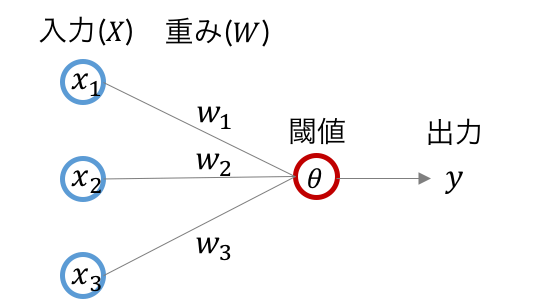
\includegraphics[width=200pt]{./img/neuron.png}
\end{center}
\caption{各ニューロンの仕組み}
\label{fig:neuron}
\end{figure}

\begin{figure}[t]
\begin{center}
\hspace*{-40pt}\makebox[1.2\textwidth][c]{
	\minipage{0.53\textwidth}
		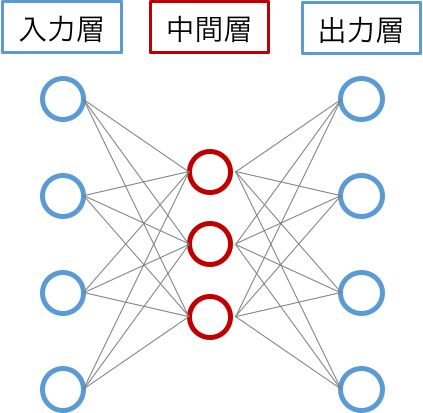
\includegraphics[height=100pt]{./img/neuralnetwork.png}
		\caption{ニューラルネットワークのモデル構造}
		\label{fig:neuralnetwork}
	\endminipage\hfill
	\minipage{0.53\textwidth}
		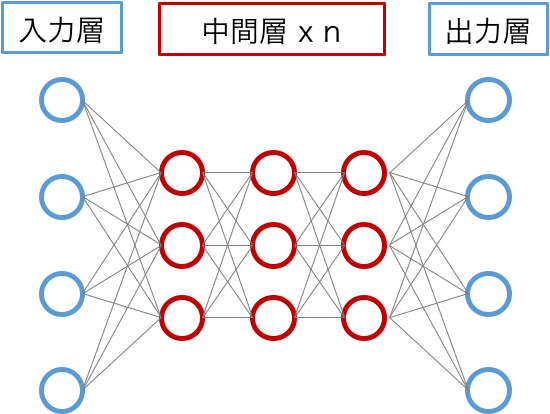
\includegraphics[height=100pt]{./img/deeplearning.png}
		\caption{深層学習のモデル構造}
		\label{fig:deeplearning}
	\endminipage\hfill
}
\end{center}
\end{figure}


各ニューロンは図\ref{fig:neuron}のようにモデル化される.
各ニューロンは他のニューロンから入力信号$x$を受け取るが,その信号の伝達効率は一様ではない.
それぞれの入力には伝達効率として重み$w$が設定され,その重み付きの入力$w x$が対象のニューロンに加算されていく.
その総和がある閾値$\theta$を超えた時,該当のニューロンは発火したものと見なし,他のニューロンに出力信号$y$が送られる.
%以上の性質は以下の式で表される.(式)


% 勾配法と活性化関数についても述べる
% 重みとバイアス項 本参考に

このようにモデル化された各ニューロンを,人間の脳の神経回路のように,互いに結合させてネットワーク化した例が図\ref{fig:neuralnetwork}である.
これは1958年にRosenblattにより提案されたパーセプトロンというネットワークで,
二ューラルネットワークの元祖とも言われる最も基本的なネットワークである\cite{rosenblatt1958perceptron}.
それぞれのニューロン(以下,ユニット)は,各層の間で互いに全結合しており,
前の層からの入力に重みが掛け合わされ,一定の閾値を超えた場合に次の層に入力が伝達される.
基本はこの構造に基づいて入出力が行われ,その結果に基づいて各重み(パラメータ)の値が修正されることで学習が進む.
単純なパーセプトロンの構造だけでは複雑な問題を捉えきれないが,
後に考案された誤差逆伝搬法\cite{rumelhart1988learning}と呼ばれる,
出力結果に基づいて,
出力を最適化するように入力層に向かって順番に重みを修正する手法により,
複雑な問題を説明するような,ユニット間の重みを学習できるようになった.


このような複雑な構造を持つニューラルネットワークは,極めて高い計算処理性能を要することが課題であった.
そのため,このモデルが考案されて以来,長い間実用には堪えない時代が続いたが,
近年の計算機の性能向上や,その他のモデル上の技術的進歩を背景に,
ニューラルネットワークをさらに多層に重ねて,より複雑な特徴を抽出し,表現できるように設計されたのが深層学習である.
深層学習モデルは図\ref{fig:deeplearning}に表されるように,複数の中間層を設けている点が,従来のニューラルネットワークとの大きな違いである.




\subsection{深層学習の概要}
% - 深層学習の5W1Hについて説明
深層学習は多層のニューラルネットワークによる機械学習のことで,
従来の機械学習では,人間が問題の特徴を捉えて素性を設計する必要があったが,
深層学習では,目的に応じた素性を,最適化の過程でデータから自動で学習することが可能である.

深層学習の活用により,
画像認識\cite{schroff2015facenet,szegedy2014going},
音声認識\cite{hinton2012deep, bahdanau2015end},
会話認識\cite{sak2015fast},
機械翻訳\cite{sutskever2014sequence, dong2015multi},
質問応答文生成\cite{yin2015neural},
画像説明文生成\cite{xu2015show,vinyals2014show}等,
多様な研究領域で飛躍的な進展が報告がされている.

特に,直近の一年間だけでも
画像から動画を生成する研究\cite{vondrick2016generating}や,
会話を人間と同程度に認識できるとする音声認識の研究\cite{xiong2016achieving},
一部の欧米言語間の文レベルで,ほぼ人間と同等に正確な翻訳を実現したとする機械翻訳の研究\cite{wu2016google}などを始めとする数々の報告がされており,
深層学習によって,日々驚異的な成果が生み出されている.

また,2016年3月に人間のプロを倒したことで一躍有名になった,Google Deep Mindが開発したコンピュータ囲碁プログラムの「AlphaGo」\cite{silver2016mastering}は,
過去の人間が打った大量の棋譜に深層学習を適用した後,コンピュータ同士の対局による強化学習を通して,
今後10年は不可能と言われていた,人間のプロを打ち負かすほどの棋力を獲得した.
AlphaGoは,過去の対局の情報である棋譜の分析によって人間を真似ただけでなく,
それまで人間が考えつかなかったような手を学習しており,囲碁界に衝撃を与えている.
このように,深層学習は,人間が認識できないようなデータの複雑な特徴を捉えることで,
これまで人間が作り上げてきた概念を,大きく塗り替える可能性を秘めている.


%大規模データが必要であることに言及
一般に,深層学習モデルを学習させる際には,大規模な訓練データが必要となる.
深層学習モデルが,人の手で素性を設計していない生の訓練データから,特徴的な表現を学習し,最適化するには,
膨大な数の内部パラメータを設定して学習することが必要で,ときには数十万から数百万以上の内部パラメータが設定されることもあり,
こうした膨大な数のパラメータを学習するには,大規模な訓練データが必要となる.
データ数が不足すると,データの潜在的な特徴を十分に学習できないことに加え,
汎用性の低い特徴まで過剰に学習してしまう「過学習」に陥りやすくなる\cite{tetko1995neural}.

実際に大規模データを利用した研究の例を挙げると,
人間より高い精度で人の顔を見分けらると報告する顔認識の研究\cite{schroff2015facenet}では,
数百万人の2億枚以上の顔画像を訓練データに利用している.
英語からフランス語に翻訳する機械翻訳の研究\cite{xu2015show}では,
1200万もの文章を訓練データとして利用している.


\subsection{Recurreut Neural Networks}
% - 特に,知識獲得の予測で用いられるRNNについて5W1H
深層学習のネットワークには,目的に応じたいくつかの種類があるが,
%特に,画像処理に利用されるConvolutional Neural Networks\cite{lecun1998gradient}というネットワークと,
%系列データの処理に利用されるRecurreut Neural Networks\cite{williams1989learning}(以下,RNN)というネットワークがよく利用される.
ここでは,知識獲得の予測に深層学習を用いた手法\cite{piech2015deep}に用いられていたニューラルネットワークである,Recurreut Neural Networks\cite{williams1989learning}(以下,RNN)について説明する.


RNNは深層ニューラルネットワークの一種で,主に系列データの解析に利用される.
系列データとは,同質のデータを直列に並べて表現することにより,特定の意味を持ったデータのことで,
例えば,時系列に沿って変化する株価のようなデータや,一定の長さで順序を持って並ぶ単語から構成される文章などのデータが系列データにあたる.

近年,RNNはデータの大規模化や計算機性能の向上などにより,幅広い領域の系列データに対して適用されるようになった.
具体的には,
機械翻訳\cite{sutskever2014sequence, dong2015multi},
手書き文字認識\cite{graves2009offline,louradour2014curriculum},
音声認識\cite{hinton2012deep,bahdanau2015end},
ユーザログ解析\cite{hidasi2015session},
画像説明文生成\cite{xu2015show,vinyals2014show},
医療診断\cite{choi2015doctor,lipton2015learning}等の領域で高い性能を発揮することが報告されている.

% - RNNの構造の概略
\begin{figure}[t]
\begin{center}
\hspace*{-40pt}\makebox[1.2\textwidth][c]{
	\minipage{0.53\textwidth}
		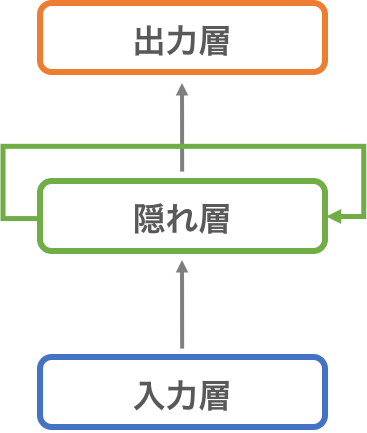
\includegraphics[height=100pt]{./img/rnn_fold.png}
		\caption{RNNの基本構造}
		\label{fig:rnn_fold}
	\endminipage\hfill
	\minipage{0.53\textwidth}
		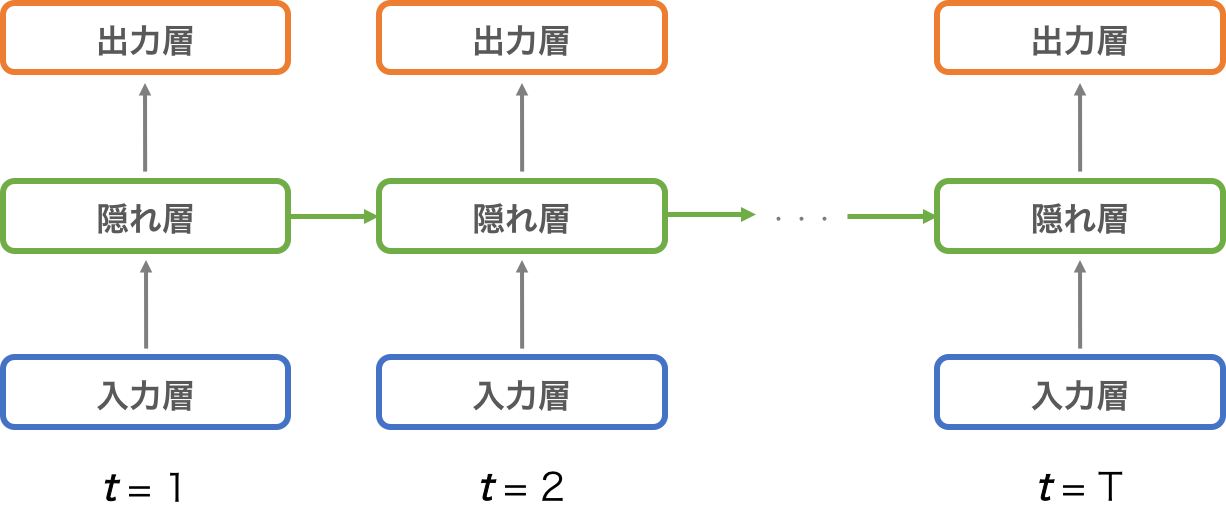
\includegraphics[height=100pt]{./img/rnn_unfold.png}
		\caption{RNNの基本構造(展開)}
		\label{fig:rnn_unfold}
	\endminipage\hfill
}
\end{center}
\end{figure}

伝統的なRNNは,
入力層,隠れ層,出力層の3層から構成されている.
系列方向を時刻とすれば,
時刻$t$の隠れ層${\bf h}_t$の計算に時刻$t-1$の隠れ層の情報を入力する${\bf h}_t = f({\bf x}_t, {\bf h}_{t-1})$という式のように,一つ前の情報を繰り返し(recurrent)入力するという構造である.
モデル構造は図\ref{fig:rnn_fold}のように表され,隠れ層の部分を時間方向に展開して図\ref{fig:rnn_unfold}のように表されることもある.
関数$f$は,入力である${\bf x}_t$や${\bf h}_{t-1}$をアフィン変換\footnote{平行移動と線形変換を組み合わせた変換のこと.}して足しあわせた後,活性化関数にかけるというものがよく利用される.
活性化関数はシグモイド関数やtanh(Hyperbolic Tangent関数),Relu\cite{nair2010rectified},ELUs\cite{clevert2015fast}など多く提案されており,通常,非線形関数である.



% - RNNの課題について説明
このように,データの系列に沿った情報を反映して学習できるRNNだが,
課題の一つとして,長期的な表現になるほど学習が難しくなるということが挙げられる\cite{bengio1994learning}.
RNNの学習には,勾配法に基づいた確率的勾配降下法\cite{robbins1951stochastic,kushner2003stochastic}やAdam\cite{kingma2014adam},AdaDelta\cite{zeiler2012adadelta}など,さまざまな手法が利用可能である.
しかし,いずれの勾配法を用いるにせよ,
勾配が爆発して学習モデルが壊れてしまうという勾配爆発\cite{bengio1994learning,pascanu2013difficulty}という問題や,
勾配が消滅して対象データの長期的な特徴量を捉えることができないという勾配消滅\cite{pascanu2013difficulty, hochreiter1998vanishing}という問題がしばしば発生する.
これは,
${\bf h}_t = f({\bf x}_t, {\bf h}_{t-1})$の式に表れるように同じ変換を繰り返し行うためであり,
このため,特に長い系列データをRNNで学習する場合,効果的に長期的な表現を学習させることが難しい.


% - 課題解決の手法について説明
こうした問題を解決もしくは緩和するため,学習時の勾配に制約を加える方法やゲート付き活性化関数の利用が提案されている.
まず,勾配爆発の緩和に対しては,学習時の勾配に制約を加える方法が有効である.
具体的には,
\cite{mikolov2012statistical}では
学習させるパラメータの勾配の絶対値の最大値を予め決めておき,
最大値以上の場合には,勾配の最大値になるように勾配の値を置き換えることで勾配爆発の影響を緩和する方法が報告された.
また,
\cite{pascanu2013difficulty}では
学習させるパラメータの勾配のノルム\footnote{ベクトルの「長さ」の概念を一般化したもの}の最大値を予め決めておき,
最大値以上の場合には, ノルムが最大値以下になるように疑似コード\ref{normregular}に従いノルムを抑制することで勾配爆発の影響を緩和する方法が報告された.
\begin{algorithm}                      
\caption{勾配爆発を防ぐための勾配ノルム抑制の疑似コード}
\label{normregular}                          
\begin{algorithmic}                  
	\STATE $\hat{{\bf g}} \leftarrow \frac{\delta \varepsilon}{\delta {\bf \theta}}$
	\IF{$\Vert \hat{{\bf g}} \Vert \geq threshold $}
	\STATE $\hat{{\bf g}} \leftarrow \frac{threshold}{\Vert \hat{{\bf g}} \Vert} \hat{{\bf g}}$
	\ENDIF
\end{algorithmic}
\end{algorithm}


次に,勾配消滅の緩和に対しては,ゲート付き活性化関数の利用が有効である.
先に言及したが,RNNには異なる活性化関数を利用するという形でいくつかの種類がある.
うまく設計された活性化関数を利用することで,勾配消滅を緩和してデータの長期的な特徴をよく捉えられたり,計算コストを削減することができたりする.
以降では,よく研究報告で取り上げられるSimple RNN(以下,SRNN)\cite{williams1989learning},Long Short  Term Momory RNN(以下,LSTM-RNN)\cite{hochreiter1997long},Gated Recurrent Neural Networks(以下,GRNN)\cite{cho2014learning}の3つについて詳細に説明する.



\subsubsection{SRNN}
SRNNはゲート付き活性化関数を用いない簡単な構造のRNNである.
\cite{le2015simple, krueger2015regularizing}で報告される工夫を取り入れることで,データの長期的な特徴を効果的に捉えることができるようになるが,
多くの場合で,LSTM-RNNやGRNNのようにゲート付き活性化関数を用いるRNNの方がモデルの性能という点で優れている.

SRNNによるモデルの定式はいくつか種類が存在するが,シンプルなものは例えば下記の式で定義される.
\begin{eqnarray}
\label{eq:srnn1}
{\bf h}_t &=& \tanh({\bf W}_{xh} {\bf x}_t + {\bf W}_{hh}  {\bf h}_{t-1} + {\bf b}_h)\\
\label{eq:srnn2}
{\bf y}_t &=& \sigma( {\bf W}_{hy} {\bf h}_t + {\bf b}_y)
\end{eqnarray}
ここでは,
$t$は時刻を指し,
${\bf x}_t$は時刻$t$の入力ベクトルを指し,
${\bf h}_t$は時刻$t$の隠れ層を指し,
${\bf y}_t$は時刻$t$の入力ベクトルを元にした予測値を指し,
${\bf W}_{xh}$,${\bf W}_{hh}$はそれぞれ重み行列を指し,
${\bf b}_h$,${\bf b}_y$はそれぞれバイアス項を指し,
$\tanh$は$( e^x - e^{-x} )/( e^x + e^{-x} )$で定義されるHyperbolic Tangent関数を指し,
$\sigma$は$1 / (1 + e^{-x})$で定義されるシグモイド関数を指す.
訓練時には,重み行列${\bf W}_{xh}$,${\bf W}_{hh}$とバイアス項${\bf b}_h$,${\bf b}_y$を学習する.


\subsubsection{LSTM-RNN}
LSTM-RNNはLong Short Term Memoryという活性化関数を用いるRNNで,
その名前の通り,SRNNでは捉えることが難しかったデータの長期的表現と短期的表現の両方の獲得を目的に開発されたものである\cite{hochreiter1997long}.
LSTM-RNNはSRNNと比較すると,モデルの性能という点で優れているが,内部のパラメータの数が非常に大きく学習コストは大きい.
最先端の成果を報告する研究でしばしば利用されているが,
LSTM-RNN自体が開発されたのは1997年でありLSTN-RNNが新しいというわけではない.

LSTM-RNNによるモデルの定式にはいくつか種類が存在するが,特に,後述するDeep Knowledge Tracing\cite{piech2015deep}で用いられるLSTM-RNNは下記の式で定義される.
\begin{eqnarray}
\label{eq:lstmrnn1}
{\bf i}_t &=& \sigma({\bf W}_{xi}{\bf x}_t + {\bf W}_{hi}{\bf h}_{t-1} + {\bf b}_i) \\
\label{eq:lstmrnn2}
{\bf g}_t &=& \sigma({\bf W}_{xg}{\bf x}_t + {\bf W}_{hg}{\bf h}_{t-1} + {\bf b}_g) \\
\label{eq:lstmrnn3}
{\bf f}_t &=& \sigma({\bf W}_{xf}{\bf x}_t + {\bf W}_{hf}{\bf h}_{t-1} + {\bf b}_f) \\
\label{eq:lstmrnn4}
{\bf o}_t &=& \sigma({\bf W}_{xo}{\bf x}_t + {\bf W}_{ho}{\bf h}_{t-1} + {\bf b}_o) \\
\label{eq:lstmrnn5}
{\bf m}_t &=& {\bf f}_t \odot {\bf m}_{t-1} + {\bf i}_t \odot {\bf g}_t \\
\label{eq:lstmrnn6}
{\bf h}_t &=& {\bf o}_t \odot {\bf m}_t  \\
\label{eq:lstmrnn7}
{\bf y}_t &=& \sigma({\bf W}_{my} {\bf m}_t + {\bf b}_y) 
\end{eqnarray}
ここでは,
${\bf i}_t$はInput Gateを指し,
${\bf f}_t$はForget Gateを指し,
${\bf g}_t$はメモリセルへの入力を指し,
${\bf o}_t$はOutput Gateを指し,
${\bf m}_t$はメモリセルを指し,
${\bf W}_{xi}$,${\bf W}_{hi}$,
${\bf W}_{xg}$,${\bf W}_{hg}$,
${\bf W}_{xf}$,${\bf W}_{hf}$,
${\bf W}_{xo}$,${\bf W}_{ho}$,
${\bf W}_{my}$
はそれぞれ重み行列を指し,
${\bf b}_i$,${\bf b}_g$,${\bf b}_f$,${\bf b}_o$,${\bf b}_y$はそれぞれバイアス項を指し,
$\odot$は要素積を指す.

式\ref{eq:lstmrnn5}にあるように,メモリセルへの入力は1つ前のメモリセルの状態${\bf m}_{t-1}$と入力${\bf g}_t$であり,
それぞれの入力に対して,過去のメモリセルからの情報を捨てるForget Gateと現在からの情報を調整するInput Gateを作用させ,${\bf m}_t$を得る.
新しい隠れ層${\bf h}_t$は式\ref{eq:lstmrnn6}のようにメモリセルからの出力をOutput Gateで調整したものを入力として受け取る.
これらのゲートにより,
長期的な特徴と短期的な特徴が捉えられるとされている.

\subsubsection{GRNN}
GRNNはGated Recurrent Unit\cite{cho2014learning}というゲート付き活性化関数を用いるRNNのことで,
GRUはLSTMのように,長期的な表現と短期的な表現を捉えるために提案された活性化関数である.
Choら\cite{cho2014learning}が2014年に発表して以来,GRNN自体やGRNNの活用に関する研究が多く報告されている\cite{chung2014empirical, zaremba2015empirical, chung2015gated, karpathy2015visualizing, biswassentiment, pezeshki2015sequence}.
LSTMよりもゲートの数が少なく学習コストが小さい傾向にあるが,
LSTM-RNN,GRNNの性能を比較した研究\cite{chung2014empirical, zaremba2015empirical}においてLSTM-RNNとGRNNが同程度の性能であることが報告されている.

GRNNは下記の式により定義される.
\begin{eqnarray}
\label{eq:grurnn1}
{\bf r}_t &=& \sigma({\bf W}_{xr}{\bf x}_t + {\bf W}_{hr}{\bf h}_{t-1} + {\bf b}_r)\\
\label{eq:grurnn2}
{\bf z}_t &=& \sigma({\bf W}_{xz}{\bf x}_t + {\bf W}_{hz}{\bf h}_{t-1} + {\bf b}_z)\\
\label{eq:grurnn3}
\tilde{{\bf h}}_t &=& \tanh({\bf W}_{xh}{\bf x}_t + {\bf W}_{hh}({\bf r}_t \odot {\bf h}_{t-1} + {\bf b}_h))\\
\label{eq:grurnn4}
{\bf h}_t &=& {\bf z}_t \odot {\bf h}_{t-1} + (1 - {\bf z}_t) \odot \tilde{{\bf h}}_t\\
\label{eq:grurnn5}
{\bf y}_t &=& \sigma( {\bf W}_{hy} {\bf h}_t + {\bf b}_y)
\end{eqnarray}
ここでは,
${\bf W}_{xr}, {\bf W}_{hr}, {\bf W}_{xz}, {\bf W}_{hz}, {\bf W}_{xh}, {\bf W}_{hh}$は重み行列で, 
${\bf b}_r, {\bf b}_z, {\bf b}_h$はバイアス項である.
${\bf r}_t$がReset Gate(LSTMにおけるForget Gateに相当する機構)で,  
${\bf z}_t$がUpdate Gate(LSTMにおけるメモリセルに相当する機構)である.
${\bf r}_t$が0に近いほど前の隠れ層からの入力よりも現在の入力をより強く考慮するようになり,
${\bf z}_t$が0に近いほど前の隠れ層をより大きく更新するようになる.


\vvspace


以上,周辺知識を整理した上で深層学習について述べ,本研究と関連の深いRNNについて詳述することで,技術的な前提知識を確認した.

次に,知識獲得の予測について述べる.



\section{知識獲得の予測}
% - 知識獲得の予測について5W1H(what, when, who, why, where, how)
知識獲得の予測は,生徒が対象の知識を獲得しているか否かを予測する問題である.
通常,知識を獲得しているか否かは問題回答の正誤を基に評価されるため,
知識獲得の予測のタスクは過去の生徒の問題回答履歴から次に解く問題の正誤を予測するというものである.

最初の定式化の事例は,1994年にCorbettらによって報告されたKnowledge Tracing\cite{corbett1994knowledge}である.
スキルの習熟学習において,
領域知識をよく分析し階層的に知識間関係を構築し,
階層構造においてより水準の高い知識に着手する前に予め獲得するべき知識が確実に獲得されるように学習体験を設計することで,
ほとんどの生徒がスキルを十分に習熟できるとする仮説\cite{keller1968good, bloom1968learning}や,
コンピュータサイエンスの発展を受けて,
予め獲得すべき知識が確実に獲得されるように生徒の知識の獲得有無を予測するというのが主な目的であった.
Knowledge Tracingにおける生徒とモデルは,生徒が勉強し知識を獲得したら,モデルが生徒が獲得した知識を予測することで生徒の獲得している知識の変化を追跡する({\it Knowledge Tracing}),という関係になっている.


% - 伝統的には2つのアプローチがあることを説明
伝統的に,知識獲得の予測には知識獲得の時系列性を重視するものと,知識間の関係性を重視するものがある.
\cite{corbett1994knowledge}で報告されたBayesian Knowledge Tracingという手法は知識獲得の時系列性を重視するもので,
問題に予めスキルを割り当て個々のスキルに習熟過程に関する4つの確率変数を定義しモデル化するというもので,
スキル間の関係性は考慮しないが,個々のスキルの習熟,つまり時系列性を考慮する手法である.
\cite{pavlik2009performance}で報告されたPerformance Factor Analysisという手法は知識間の関係性を重視するもので,
個々の知識(あるいは,スキル)に関する過去の回答の正誤を重み付けして,次の問題の正誤を予測しようというもので,
Performance Factor Analysisは知識獲得の時系列性より知識間の関係性を重視する手法である.
いずれの手法も本論文と関連が深い.


以降では,まず,Knowledge Tracingの定式化について述べ,
Bayesian Knowledge TracingとPerformance Factor Analysisの2つの手法を説明し,
最後に,深層学習を活用したDeep Knowledge Tracingについて説明する.


\subsection{Knowledge Tracingの定式化}
Knowledge Tracingは過去の生徒の問題回答履歴から生徒が次に解く問題の正誤を予測するというものである.
生徒の時刻$t$において観測された問題回答結果を$q_{t}$とすれば,
$q_1, q_2, \dots, q_t$から時刻$t+1$において観測される問題回答結果$q_{t+1}$を予測するタスクと表現できる.
特に,過去の観測された問題の正誤から将来の正誤確率を算出する場合は,
$q_1, q_2, \dots, q_t$が観測された場合の時刻$t+1$に着手する問題において当該生徒の回答正解となる事後確率
$p(q_{t+1} = correct|q_1, q_2, \dots, q_t)$を求めるタスクであるといえる.
予測性能の評価は\cite{yudelson2013individualized, falakmasir2015spectral}ではAccuracy\footnote{正解率.予測結果全体と、答えがどれぐらい一致しているかを判断する指標.0〜1で表され,完全な予測時に1となる.}で,
\cite{piech2015deep}ではAUC\footnote{正例を正しく分類した割合を縦軸に,負例を正しく分類した割合を横軸に取るROC曲線における,曲線より下の面積.0〜1で表され,完全な予測時に1となり,ランダムな予測で0.5付近を示す.}で行っており,
目的に応じてさまざまである.
本研究では,AUCによって予測性能を評価する.


なお,モデルの入力となる「問題」の粒度はさまざまである.
問題への回答の結果は,その問題を回答するのに必要な知識を生徒が獲得しているか否かを評価するという点で,
知識集合を表現しており,また,その粒度もさまざまである.
個々の問題をそのままモデルの入力次元とするものや,問題に予めタグを割り当て問題により評価される知識の粒度をある程度整え,そのタグをモデルの入力次元とすることもある.
例えば,
\cite{piech2015deep}ではモデルの入力次元は演習タグもしくはスキルタグと呼ばれるものであり,
演習問題に割り当てられ,それぞれの演習問題で扱われる知識の要素を説明するものである.
通常,こうしたタグは専門家によって設計され,利用される.
本論文では,個々の問題をそのままモデルの入力次元として用いる.


\subsection{Bayesian Knowledge Tracing}
Bayesian Knowledge Tracing\cite{corbett1994knowledge}(以下,BKT)はベイズの定理の事前確率と事後確率の関係に基づいて正解確率$p(q_{t+1} = correct|q_1, q_2, \dots, q_t)$をモデリングする手法である.
BKTには下記の4つの確率変数がある.
\begin{itemize}
\item 初めから当該スキル理解している確率$p(L_0)$(もしくは $p\mhyphen init$)
\item 生徒が当該スキルを理解していない状態から理解している状態へ遷移する確率$p(T)$(もしくは $p\mhyphen transit$)
\item 生徒が当該スキルを理解しているが誤答する確率$p(S)$(もしくは $p\mhyphen slip$)
\item 生徒が当該スキルを理解していないが推測で正解する確率$p(G)$(もしくは $p\mhyphen guess$)
\end{itemize}
これらの4つの確率変数がすべてのスキルに定義されている.つまり,スキル数を$N$とすれば,確率変数の合計数は$4N$である.
生徒$u$がスキル$k$の問題を時刻$t$に解いた場合に正解する確率は下記の式に基づいて更新される.

\hspace*{-55pt}\minipage{1.1\textwidth}
\begin{eqnarray}
\label{eq:bkt_update1}
p(L_1)^{k}_{u} &=& p(L_0)^k \\[\eqnsp]
\label{eq:bkt_update2}
p(L_{t}|obs=correct)^{k}_{u} &=& \frac{ p(L_{t-1})^{k}_{u} \cdot (1 - p(S)^k) }{ p(L_{t-1})^{k}_{u} \cdot (1 - p(S)^k) + (1 - p(L_{t-1})^{k}_{u}) \cdot p(G)^k } \\[\eqnsp]
\label{eq:bkt_update3}
p(L_{t}|obs=wrong)^{k}_{u} &=& \frac{ p(L_{t-1})^{k}_{u} \cdot p(S)^k }{ p(L_{t-1})^{k}_{u} \cdot p(S)^k + (1 - p(L_{t-1})^{k}_{u}) \cdot (1 - p(G)^k) } \\[\eqnsp]
\label{eq:bkt_update4}
p(L_{t})^{k}_{u} &=& p(L_{t}|obs)^{k}_{u} + (1 - p(L_{t}|obs)^{k}_{u}) \cdot p(T)^k  \\[\eqnsp]
\label{eq:bkt_update5}
p(C_{t})^{k}_{u} &=& p(L_{t-1})^{k}_{u} \cdot (1 - p(S)^k) + (1 - p(L_{t-1})^k_{u}) \cdot p(G)^k
\end{eqnarray}
\endminipage\hfill
%}
\vvspace
\vvspace


右上の$k$はスキル番号を示し,右下の$u$はユーザ番号を示すことに注意されたい.
まず,生徒$u$が初めから当該スキル$k$を身につけている確率は式\ref{eq:bkt_update1}の通り定義する.
正解が観測され,正しく当該スキルを身につけている確率は,式\ref{eq:bkt_update2}で与えられ,
不正解が観測されたが,正しく当該スキルを身につけている確率は,式\ref{eq:bkt_update3}で与えられ,
それらを合わせて,次の時刻に当該スキルを身につけている確率は,式\ref{eq:bkt_update4}で与えられる.
このように定めることで,理解しているがうっかり間違ってしまう場合や, 理解していないがあてずっぽうで正解してしまう場合を考慮できる.
なお当該モデルでは,身につけたスキルの忘却は無視している.
最後に,生徒$u$がスキル$k$の問題を時刻$t$に解いた場合に正解する確率$p(C_{t})^{k}_{u}$は式\ref{eq:bkt_update5}のように算出され,
この値を次の問題の正誤予測に利用する.
 
上記に説明したモデルの学習にはいくつかの方法が適用され報告されている.
1つは\cite{corbett1994knowledge}にあるように隠れマルコフモデル(HMM)を用いて生成モデルとして学習させる方法であり,
1つは\cite{yudelson2013individualized}にあるように勾配法を用いて識別モデルとして学習させる方法である.
それぞれ長所と短所があるが,
特に,大規模データへの適用という観点ではHMMに基づいた生成モデルの手法では計算量が大きく学習に非常に多くの時間がかかってしまうということもあり,
\cite{yudelson2013individualized}では勾配法に基づいた識別モデルとして学習させている.
具体的には,\cite{yudelson2013individualized}では,目的関数に負の対数尤度(Negative Log Likelihood)を利用し,勾配降下法(Gradient Descent)で学習させている.
%本論文で扱うデータは大規模であるため,学習方法は識別モデルとして扱う場合について説明した.
%生成モデルとして扱う場合の学習方法については\cite{corbett1994knowledge}を参照されたい.



\subsection{Performance Factor Analysis}
Performance Factor Analysis\cite{pavlik2009performance}(以下,PFA)も
過去の生徒の問題回答履歴から生徒が次に解く問題の正誤を予測するための手法である.
しかし,
知識獲得の時系列性を考慮するBKTと異なり,
知識獲得の順番を考慮せず知識間の関係性を考慮して予測する手法である.
PFAは下記のように定義される.
\begin{eqnarray}
	p(i, j \in KCs, s, f) & = & \sigma( \beta _j + \sum_{k \in KCs}(\gamma_k s_{i, k} + \rho _k f_{i, k}) )
\end{eqnarray}
ここでは,
$s$は事前に正答した問題回答,
$f$は事前に誤答した問題回答,
$p$はユーザ$i$が知識$j$に正答する確率,
$\beta_j$は知識$j$の簡単さ,
$\gamma_k$と$\rho_k$はそれぞれ知識$k$の正答と誤答の重み,
$s_{i, k}$と$f_{i, k}$はそれぞれユーザ$i$が知識$k$に事前に正答した問題回答,事前に誤答した問題回答
である.
$\sigma$はシグモイド関数,
過去の各知識の正誤を重み付けしシグモイド関数にかけ,別の問題の正誤を予測するというものである.

%特に,深層学習を用いる前のKnowledge Tracingでは
%問題回答の順番を考慮していたが知識間の関係性は考慮する研究は著者の知る限り\cite{kaser2014beyond}の以外ない.
PFAは
知識間の関係性を考慮できない場合に複数の知識がないと獲得できない知識のモデルが難しいという
Bayesian Knowledge Tracingやその拡張手法の問題を解決するために
提案された.
PFAは知識間の関係性を重み付けして考慮しているが,
問題回答の順番は考慮しない.


\subsection{Deep Knowledge Tracing}
Deep Knowledge Tracing\cite{piech2015deep}(以下,DKT)はRNNを利用しKnowledge Tracingを行う手法である.
2015年6月に発表された.
数学の問題回答ログのデータセットで実験され,
高い性能で将来の知識獲得を予測できること,
予測モデルを分析することで知識間関係をネットワークとして抽出できることが報告された.
生徒が獲得している知識から,ある知識の獲得されやすさをそのまま予測しており,
得られた知識間関係から抽出されたネットワークは知識獲得における知識構造を表現しているといえる.
DKTの構造と最適化,および知識間関係の抽出手法について順に説明していく.



\subsubsection{構造}
まず,DKTの構造について述べる.
DKTの構造は伝統的なRNNの構造に基づいている.
伝統的なRNNは入力のベクトル系列${\bf x}_1, \dots, {\bf x}_T$を出力のベクトル系列${\bf y}_1, \dots, {\bf y}_T$に写像する.
この写像は,隠れ状態${\bf h}_1, \dots, {\bf h}_T$を計算することで達成されるが,一連の写像の過程で過去観測から得られる関連情報を将来予測のために連続的に符号化している,とみなせる.確率変数は下記の式で定義されるネットワークにより関連付けられる.
\begin{eqnarray}
\label{eq:rnn1}
{\bf h}_t &=& f({\bf x}_t, {\bf h}_{t-1})\\
\label{eq:rnn2}
{\bf y}_t &=& g({\bf h}_t)
\end{eqnarray}
モデルは関数$f$と$g$によって定義されており,
これらの関数$f, g$にはSRNNの式\ref{eq:srnn1},\ref{eq:srnn2}やLSTM-RNNの式\ref{eq:lstmrnn1}--\ref{eq:lstmrnn7},GRNNの式\ref{eq:grurnn1}--\ref{eq:grurnn5}を利用できる. 


RNNで生徒の学習行動の観測結果をモデリングするため観測結果を固定長の入力ベクトル${\bf x}_t$の系列に変換する必要があるが,DKTではシンプルな変換を行っている.具体的には,生徒の学習行動の観測結果をone-hotベクトルに符号化し${\bf x}_t$とする,というものである.
観測結果は演習問題と正誤の組み合わせで表現できるため,演習問題の数を$M$とすれば,${\bf x}_t$の長さは$2M$となる.


\begin{table}[ht]
\caption{Deep Knowledge Tracingにおける回答ログデータと対応する入力ベクトルの例}
\label{tab:samplelog}
\begin{center}
\centerline{
{
\begin{tabular}{crrr|cc}\hline\hline
	\multicolumn{4}{c|}{回答ログ}	&	\multicolumn{2}{c}{入力ベクトル}	\\
	ユーザID	&	ログの順番	&	問題番号	&	正誤	&	変数名			&	値											\\\hline
	A			&	1			&	1			&	0		&	${\bf x}_1$ 			& $[0 0 0 0 \vdots 1 0 0 0 ]$	\\
	A			&	2			&	1			&	1		&	${\bf x}_2$ 			& $[1 0 0 0 \vdots 0 0 0 0 ]$	\\
	A			&	3			&	2			&	1		&	${\bf x}_3$ 			& $[0 1 0 0 \vdots 0 0 0 0 ]$	\\
	A			&	4			&	3			&	0		&	${\bf x}_4$ 			& $[0 0 0 0 \vdots 0 0 1 0 ]$	\\
	A			&	5			&	3			&	1		&	${\bf x}_5$ 			& $[0 0 1 0 \vdots 0 0 0 0 ]$	\\
	A			&	6			&	4			&	1		&	${\bf x}_6$ 			& $[0 0 0 1 \vdots 0 0 0 0 ]$	\\
\hline\hline
\end{tabular}
}
}
\end{center}
\end{table}


具体例を交えて説明する.
例えば,演習問題の数が4つで,問題回答は1つずつしかできないと仮定する .$M=4$であり,${\bf x}_t$の長さは$8$である.
ある生徒が,表\ref{tab:samplelog}の回答ログように問題を回答し正誤が観測されたとする.
この時に,例えば,表\ref{tab:samplelog}に記載のような入力ベクトルの系列となる.
このようにして,回答行動の観測結果を符号化することで,どの演習問題をいつ正解もしくは不正解したのかをRNNに入力できる.

出力${\bf y}_t$は問題と同じ長さのベクトルで,
それぞれの要素が当該生徒がそれぞれの問題に正しく回答する確率の予測値となっている.
したがって,$t+1$の回答$q_{t+1}$の正誤予測は$t+1$に回答される問題$q_{t+1}$に対応する${\bf y}_t$の要素から読み取れる.


\subsubsection{最適化}
次に,DKTの最適化について述べる.
訓練時に用いられる目的関数は,
モデルにおいて生徒の回答行動の観測系列の負の対数尤度(Negative Log Likelihood)である.
${\bf \delta}(q_{t+1})$を時刻$t+1$にどの問題が回答されたかのone-hotベクトルとし,
$a_{t+1}$を時刻$t+1$に当該問題で正答したか否か($1$か$0$)とし,
$l$を交差エントロピー誤差とすれば,
当該予測結果に対する損失関数は $l({\bf y}^T {\bf \delta}(q_{t+1}), a_{t+1})$であり,
生徒一人の損失関数は下記の式で与えられる.
\begin{eqnarray}
L &=& \sum_t l({\bf y}_t^T {\bf \delta}(q_{t+1}), a_{t+1})
\end{eqnarray}


学習時はミニバッチごとに確率的勾配降下法で目的関数を最小化する.
\cite{piech2015deep}では,モデル学習時には過学習を防ぐため${\bf y}_t$への入力としての${\bf h}_t$にはdropout\cite{srivastava2014dropout}を適用している(${\bf h}_{t+1}$の方向にはdropoutを適用しない).
また,系列方向の誤差逆伝搬\cite{werbos1990backpropagation}において勾配が爆発するのを防ぐため,閾値以上のノルムの勾配は\cite{pascanu2013difficulty}にしたがい,制約を設けている.


\subsubsection{知識間関係抽出法}
次に,DKTのモデルを利用した知識間関係(あるいは,問題間関係)抽出法について述べる.
DKTのモデルは,従来ではよく人間の専門家が行っていたデータの潜在的な構造や概念を発見するタスクに応用できる.
問題$i$と$j$のすべての有向ペアのうち下記の条件を満たすものに対して下記の影響度$J_{ij}$を割り当てる.\\
\begin{itemize}
	\item [条件]有向ペア$(i, j)$について,問題$i$が出現した後に残りの問題系列の中で問題$j$が出現する系列数が問題$i$が出現する問題系列数全体の$V\%$以上であること.
	\item[影響度]
$$J_{ij} = \frac{y(j|i)}{\sum_k y(j|k)}$$\\
\end{itemize}
ここでは,$y(j|i)$は,ある生徒が最初に問題$i$に正答した場合に,RNNによって割り当てられる次の時刻に問題$j$に正答する確率である.
\cite{piech2015deep}では,問題間影響行列からのネットワーク抽出には,
$V=1$を用いた.
また,ネットワークの可視化に際しては,影響度が$0.1$以上であればエッジを引くというようにしてネットワークを構築した.

さらに,\cite{piech2015deep}は,
得られたネットワークは,
単に生徒の問題$(i, j)$間の遷移率から構築したネットワークや
問題$i$の正解が観測された後に問題$j$の正解が観測される条件付き確率から構築したネットワークより
よく知識間関係を捉えていることを指摘している.


こうして得られた行列$J$は,
問題$i$で評価される知識が既に獲得されている場合に,
問題$j$で評価される知識の獲得されやすさを表現しており,
$J$は知識間関係行列であるといえ,
この知識間関係行列から構築したネットワークは
知識獲得における知識構造を表現していると考えられる.


\subsection{知識獲得予測の手法におけるDKTの最適性}

ここまで知識獲得予測の様々な手法について述べたが,
DKTを拡張する手法が,本研究の目的を達成する上で最適な手法であることを,以下の二点に基づいて説明する.

\begin{enumerate}
	\item 知識間の関係性は,知識獲得予測の文脈において,定量的に検証されて抽出されるべきこと,
	\item 知識獲得予測は,複数の知識間の影響関係や,知識獲得の時系列性を考慮して行われるべきこと,
\end{enumerate}

まず,1について述べる.
知識間の関係性は,知識獲得予測の過程で抽出されるものと,そうでないものがある.
後者については,
専門家が作成するという手法や,
テキスト解析により概念関係ネットワークを構築するという手法\cite{chen2008mining}がある.
しかし,これらの手法は,
専門家や研究者が立てた仮説に基づいた定性的なものであり,
実際の生徒の学習過程をよく説明するものであるという定量的な根拠はない.

問題回答正誤の分析により知識の構造化を行う方法[参考文献引用]も,%詳述
2つの問題$i$と$j$の間で問題$i$が正解後と不正解後の問題$j$の正解率の差と着手順序を基に知識を構造化するが,
この手法は2つの問題$i$と$j$の関係性のみを考慮しており,他の問題との関係性は独立だと見なされている.
得られた知識間関係は2つの知識の間についてのものを線形に合算したものであり,
複雑で密接に関係している複数の知識の獲得順序や影響関係を捉えているものではない.

一方で,知識間の関係性の抽出を,知識獲得を予測する過程で行うものは,
生徒の知識状態と行動を元に,知識の獲得を予測しているため,
生徒の学習過程を反映した知識間関係を表現している可能性が高い.

したがって,
知識間関係を定量的に抽出する手法としては,
知識獲得を予測する過程で知識間関係を抽出する手法に絞る.


次に,2について述べる.
知識獲得予測には,
複数の知識の影響関係や知識獲得の時系列性を考慮するものと,そうでないものがある.
% BKT的なものとDKT的なものがある
後者については,
複数の知識を独立なものとして,それらの状態の遷移を定義するBayesian Knowledge Tracing(BKT)の手法や,
過去の回答の結果を1つにまとめて定義するPerformance Factor Analysis(PFA)の手法などがある.
しかし,BKTの手法は,複数の知識を独立なものとして捉えるため,複数の知識からなる複雑な知識状態を捉えきれず,
また,PFAの手法は,直前の回答も十分な時間が立った後の回答も,一つの過去の回答として捉えるため,
生徒の時間に沿った知識獲得の状態を,現実的に捉えきれていない.

一方,DKTは,時系列に沿ってRNNの隠れ層を更新することにより,
複数の知識間の影響関係や,知識獲得の時系列性を考慮して知識獲得を予測しているので,
より現実に沿った知識間関係を抽出できる可能性が高い.

現に\cite{piech2015deep}で,
既にDKTによって知識間関係を抽出できることが報告されており,
複雑で密接に関係している複数の知識の獲得順序や影響関係を捉えている可能性が高く,
DKTを利用することが最適であると考えられる.

% PFAについては述べる必要ないかも
また,PFAとDKTのいずれの手法も知識間関係を考慮して予測に利用しているが,DKTの方が有効性が高いと考える.
なぜなら,
\cite{piech2015deep}では言及されていなかったが,
DKTはPFAの拡張になっているためである.
DKTはRNNを利用しており,
\begin{eqnarray}
{\bf h}_t & = & f({\bf x}_t, {\bf h}_{t-1})\\
{\bf p}_t & = & \sigma({\bf h}_{t-1} \cdot {\bf W}_{hp} + {\bf b}_p)
\end{eqnarray}
で与えられる.
一方でPFAは
\begin{eqnarray}
	p(i, j \in KCs, s, f) & = & \sigma( \beta _j + \sum_{k \in KCs}(\gamma_k s_{i, k} + \rho _k f_{i, k}) )
\end{eqnarray}
で与えられる.
したがって,
\begin{eqnarray}
\label{eq:discussion-func}
	f({\bf x}_t, {\bf h}_{t-1}) &=& {\bf x}_t + {\bf h}_{t-1}\\
	{\bf h}_{0} & = & [0, 0, \cdots , 0]
\end{eqnarray}
とすると,
${\bf h_t}$がこれまでの各問題についての正答回数を表現するベクトルと各問題についての誤答回数を表現するベクトルを結合したベクトルになるが, 
これは,ベクトル${\bf s}$と${\bf f}$を結合したものと同じである.
したがって,
PFAはDKT内部のRNNの繰り返しの部分を表現する関数$f$を式\ref{eq:discussion-func}にした特殊なケースであり,
DKTはPFAの拡張になっている.

\vvspace
以上,知識獲得の予測研究について述べ,本研究の素地となっている研究について整理した.
次に,次元削減手法について述べる.


\section{次元削減手法}
高次元のデータから低次元の特徴表現を抽出する,次元削減手法について述べる.
本研究が目的とする知識分類表現の抽出は,一般的な次元削減の手法を拡張したものであり,
一般的な次元削減手法について説明することで,
基礎となる知識や本研究との差分を明確にすることを目的とする.


一般に,機械学習や統計においては,扱うデータの次元が大きい場合に,次元削減を行うことが多い.
これは,データの次元が大きすぎることにより,データのサンプル数に対してモデルが複雑化してしまい,認識精度が悪くなる「次元の呪い」\cite{bellman1957dynamic,friedman1997bias}という現象を回避する目的の他,
可読性を高めることにより,人間が解釈しやくすることなどを目的としている.
知識獲得予測において用いられる知識分類も,
分類のなされていない生の問題は次元数が大きく,そのままでは人間が解釈したり教育に用いることが困難なため,
内容や難易度の類似度など,一定の尺度に従って,人間の手により次元削減が行われた例である.
本研究ではこうした次元削減を,人間の手ではなく深層学習によって行うことで,最適化することを目的としている.


本節では,機械学習が現れる以前から一般的に使用されていた次元削減手法の代表であるPrincipal Component Analysisや,
ニューラルネットワークを活用した次元削減手法であるAutoencoder,
そして,深層学習の過程で行われるEmbeddingと呼ばれる埋め込み手法を取り上げ,
次元削減の手法について概観する.

\subsection{Principal Component Analysis}
Principal Component Analysisは,日本語では主成分分析と訳される.
相関のある多数の変数の中から,分散の大きい変数をデータ全体を説明する上で重要な「主成分」と見なし,
順にそれまでの主成分と直行するように主成分を定める変換を繰り返し行うことで,
変数間の相関をなくし,重要度の高い主成分のみを採用し,次元削減を行う手法である.

その由来は古く,1901年に力学の分野において初めて導入された\cite{pearson1901liii}ことをきっかけに,
以後,経済学や統計学,機械学習などの分野で幅広く利用されてきた\cite{wold1987principal,ku1995disturbance}.

一般的なアルゴリズムを以下に示す.

元のデータを${\bf X}$,データの次元を$M$,変換後の次元を$N$,とすると、
\begin{enumerate}
	\item データの共分散行列を求める. 
	\item 共分散行列の固有値と固有ベクトルを求める. 
	\item 固有値の大きい順に,対応する固有ベクトルを並べ替え,$N$個の固有ベクトルを並べた行列${\bf P}$を作る. 
	\item データからその平均ベクトルを引いたデータを${\bf X}_{bar}$とし,以下の式に基づいてデータを変換する. 
	\begin{equation}
		{\bf X}_{pca} = {\bf X}_{bar} {\bf P}
	\end{equation}
\end{enumerate}

主成分分析には様々な拡張がある\cite{scholkopf1997kernel,tipping1999probabilistic}が,その根底にある数学的な意味は,固有値問題を解くことにある.
固有値問題とは、ある行列${\bf A}$について、
\begin{equation} 
{\bf A} {\bf x} = \lambda {\bf x}
\end{equation} 
となるような固有値$\lambda$と固有ベクトル${\bf x}$を求めることである.
%このように,数学において一般的に定式化できる性質に基づいていることから,普遍性が高く,幅広い領域で利用されている.




\subsection{Autoencoder}
Autoencoderは,日本語では自己符号化器と訳される.
1980年代から考案されていたが,2006年の\cite{hinton2006reducing}らの研究によって広く普及した.
様々な種類のものが考案されているが,
基本的な概念は,
ニューラルネットワークに入力されたデータを一旦低次元で表現し,
その低次元表現から再び入力である自身を再現するように学習させることで,
データの特徴を適切に表す低次元表現を獲得することを目的としている.
教師データが存在しないが,自身を教師データとして行う教師あり学習のような形を取っており,
教師あり学習と教師なし学習の中間に位置するような概念として理解されることもある.


具体的な定式化について述べる.
まず,入力層$x \in \mathbb{R}_d$
に対して,以下の式によって隠れ層$h$と復元層$x^r$を定義する.
\begin{eqnarray} 
\label{eq:autoencoder_hidden}
h &=& f_\theta(x) = s({\bf W} x + b)\in\mathbb R_{d_h}
\\
\label{eq:autoencoder_reconstruct}
x^r &=& g_{\theta’}(h) = s_r({\bf W’} h + b')\in\mathbb R^d
\end{eqnarray} 

ここで,$\theta=({\bf W}, b), \theta'=({\bf W'}, b')$は学習されるパラメータであり,
$s, s_r$は活性化関数である.
こうして定義された復元層$x_r$が入力層$x$にできるだけ近づくように,
訓練データ${\bf D} = x_1, \cdots, x_n$に対する損失関数の平均値を最小化する過程で,パラメータ$\theta, \theta'$を学習する.
\begin{equation}
\label{eq:autoencoder_loss}
{\min_{\theta, \theta'} {1\over n}\sum_{i=1}^n L(x_i, g(f(x_i)))}
\end{equation}

式\ref{eq:autoencoder_loss}で表される損失関数は,一般に再構成誤差(Reconstruction Error)と呼ばれる.
損失関数$L$は,入力がバイナリ値ならば交差エントロピー誤差,実数値ならば二乗誤差を用いるのが一般的であり,%説明する? 
本研究においては,入力は問題回答の正誤を意味するバイナリ値なので,交差エントロピー誤差を用いる.

% 具体的な式
活性化関数が恒等写像,つまり活性化関数が存在せず,損失関数が二乗誤差の場合はPCAと等価になることが知られており[参考文献],
Autoencoderは,ニューラルネットワークの構造と非線形の活性化関数を用いることにより,
PCAの拡張を行っていると見なすことができる.

このように,次元削減を非線形に行うことができるAutoencoderだが,
深層学習が発達した今日では,深層学習モデルの各ユニットに良い初期値を与えるための事前学習として利用されることが多い\cite{erhan2010does}.
より頑健な特徴表現を獲得させるためにデータにノイズを加えるDenoising Autoencoder\cite{vincent2008extracting}や,
潜在的な特徴表現の分布に特定の確率分布が存在すると仮定するVariational Autoencoder\cite{kingma2014semi}など,様々な工夫が考案されている.



\subsection{Embedding}
Embeddingは,日本語では埋め込みと訳される.
一般に,ニューラルネットワークにおいて入力データの次元数が大きい場合,
そのままデータを入力すると,データの特徴的な表現について学習がしにくくなることがある.
そのため,一度次元数の少ない層へ埋め込みを行い,データのより特徴的な表現を抽出した上で学習を進めることで,精度が向上する場合があることが知られている[参考文献?].

学習後のモデルにおける埋め込み層は,入力データを低次元で表現する上で最適な特徴表現となっている可能性が高く,
この表現を抽出することでデータの特徴を保ったまま次元削減を行うことができる.


\vvspace


最後に,以上の関連研究を踏まえて,
本論文で使用する類似の用語について定義を明確にする.

\section{用語の定義}
本節では,
本論文で用いられる類似した用語の定義を行い,意味上の違いを明確にすることで,
以降の手法の説明を含めた本論文の展開を明確にすることを目的とする.

\subsection{知識獲得予測と回答正誤予測}
一般にKnowledge Tracingと呼ばれ,本研究が問題提起を行っているのは「知識獲得予測」である.
しかし,本研究は従来の「知識獲得予測」が「知識」の定義として用いている知識分類を所与のものとせず,
問題の回答ログのみを入力に用いて,その回答の正誤予測を最適化する過程で適切な知識分類を学習することを目的としている.
よって,知識分類を学習する段階では,まだ「知識」の定義はなされていないため,
この段階では正確性を期すために「回答正誤予測」という単語を用いる.

一方,学習によって得た知識分類を用いて既存の知識分類と比較を行う際には,
既に「知識」の定義がなされているため,一般的な「知識獲得予測」の単語を用いる.

\subsection{知識分類と知識タグ}
本研究で扱うデータセットには,既存の「知識分類」が存在する.
問題に対して事前に分割されている知識ごとの分類や,そのような状況を「知識分類」と呼び,
生徒が回答する各問題に紐づき,その内容を指し示す1つ1つの具体的なタグのことを「知識タグ」と呼ぶ.
指し示している状況は似ているが,
問題全体が事前に分類されている状況を意図するときは「知識分類」の単語を,
より個別の問題に紐づく具体的なタグを意図するときは「知識タグ」の単語を使用する.



以上,関連研究について述べ,本研究の学術的位置付けや周辺概念を俯瞰した.

次に,分析手法について述べる.




